\subsection{Τίτλος Υποκεφαλαίου}

\bigskip

\subsubsection{Τίτλος \ldots}

\bigskip

\subsubsection{Τίτλος \ldots}

\bigskip

% Παράδειγμα: δεύτερο διάγραμμα
\begin{diagram}[H]
  \centering
  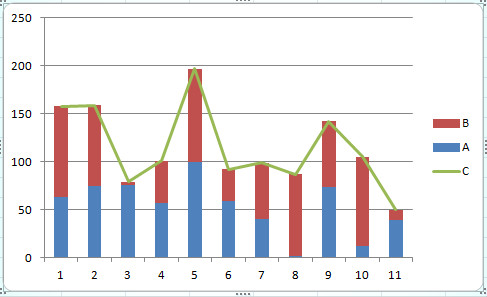
\includegraphics[width=0.7\textwidth]{images/diagram-4.2.jpg}
  \caption{Δεύτερο διάγραμμα}
  \label{diag:4.2}
\end{diagram}

\subsubsection{Τίτλος \ldots}

\bigskip

% Παράδειγμα: δεύτερος πίνακας δεδομένων
\begin{table}[H]
  \centering
  \caption{Δεύτερος πίνακας}
  \label{tab:4.2}
  \begin{tabular}{lccc}
    \toprule
    \textbf{Είδος} & \textbf{Τιμή 1} & \textbf{Τιμή 2} & \textbf{Τιμή 3} \\
    \midrule
    Α & 0.93 & 1.28 & 2.47 \\
    Β & 0.82 & 1.39 & 2.89 \\
    Γ & 0.75 & 1.32 & 3.14 \\
    \bottomrule
  \end{tabular}
\end{table}
